
\documentclass[letterpaper,12pt]{article}

\usepackage{threeparttable}
\usepackage{geometry}
\geometry{letterpaper,tmargin=1in,bmargin=1in,lmargin=1.25in,rmargin=1.25in}
\usepackage[format=hang,font=normalsize,labelfont=bf]{caption}
\usepackage{amsmath}
\usepackage{mathrsfs}
\usepackage{multirow}
\usepackage{array}
\usepackage{delarray}
\usepackage{listings}
\usepackage{amssymb}
\usepackage{amsthm}
\usepackage{lscape}
\usepackage{natbib}
\usepackage{setspace}
\usepackage{float,color}
\usepackage[pdftex]{graphicx}
\usepackage{pdfsync}
\usepackage{verbatim}
\usepackage{placeins}
\usepackage{geometry}
\usepackage{pdflscape}
\synctex=1
\usepackage{hyperref}
\hypersetup{colorlinks,linkcolor=red,urlcolor=blue,citecolor=red}
\usepackage{bm}


\theoremstyle{definition}
\newtheorem{theorem}{Theorem}
\newtheorem{acknowledgement}[theorem]{Acknowledgement}
\newtheorem{algorithm}[theorem]{Algorithm}
\newtheorem{axiom}[theorem]{Axiom}
\newtheorem{case}[theorem]{Case}
\newtheorem{claim}[theorem]{Claim}
\newtheorem{conclusion}[theorem]{Conclusion}
\newtheorem{condition}[theorem]{Condition}
\newtheorem{conjecture}[theorem]{Conjecture}
\newtheorem{corollary}[theorem]{Corollary}
\newtheorem{criterion}[theorem]{Criterion}
\newtheorem{definition}{Definition} % Number definitions on their own
\newtheorem{derivation}{Derivation} % Number derivations on their own
\newtheorem{example}[theorem]{Example}
\newtheorem{exercise}[theorem]{Exercise}
\newtheorem{lemma}[theorem]{Lemma}
\newtheorem{notation}[theorem]{Notation}
\newtheorem{problem}[theorem]{Problem}
\newtheorem{proposition}{Proposition} % Number propositions on their own
\newtheorem{remark}[theorem]{Remark}
\newtheorem{solution}[theorem]{Solution}
\newtheorem{summary}[theorem]{Summary}
\bibliographystyle{aer}
\newcommand\ve{\varepsilon}
\renewcommand\theenumi{\roman{enumi}}
\newcommand\norm[1]{\left\lVert#1\right\rVert}

\begin{document}

\title{Math 320 Homework 5.5}
\author{Chris Rytting}
\maketitle
\subsection*{5.20}
Let \[j, k, n \in \mathbb{N}, \quad \omega = e^{i\pi/n}\] 
Note that 
\begin{align*}
\Re(\omega^{k(n+j)}) &= \Re(e^{i\pi/n*k(n+j)}\\ &= \Re(e^{\frac{i\pi kn + i \pi kj}{m}})\\ &= \cos\left(\frac{\pi k n + \pi k j}{n}\right) \\&= \cos\left(\pi k  + \frac{\pi k j}{n}\right) 
\end{align*}
Now let $x = \frac{\pi k j}{n}$. If $k$ is even, we have that
\begin{align*}
\cos(\pi k + x) &= \cos(x) \\&= \cos(-x) \\&= \cos(\pi k - x) \\&= \cos(\pi k - \frac{\pi k j}{n})
\\&=\cos(\frac{\pi k n - \pi k j}{n} \\&= \Re(e^{\frac{i \pi k n - i \pi k j}{n}}) \\&= \Re(e^{\frac{i \pi}{n}*k(n-j)}) \\&= \omega ^{k(n-j)}
\end{align*}
Now if $k$ is odd we get
\begin{align*}
\cos(\pi k + x) &= \cos(\pi + x) \\&= \cos(\pi -x) \\&= \cos(\pi k - x) \\&= \cos(\pi k - \frac{\pi k j}{n})
\\&= \cos(\frac{\pi k n - \pi k j}{n}) \\&= \Re(e^{\frac{i \pi k n - i \pi k j}{n}}) \\&= \Re(e^{\frac{i \pi}{n}*k(n-j)}) \\&= \omega ^{k(n-j)} 
\end{align*}

\subsection*{5.21}
Given $n \in \mathbb{N}$, let $a_{n+j} = a_{n-j}$, and
\[c_k = \frac{1}{2n} \sum_{j = 0}^{2n-1}a_j \omega_{2n}^{-jk}\]
It suffices to show that the imaginary parts of $c_k$ sums to zero, or more precisely:
\[i\sum_{j = 0}^{2n-1}a_j(\sin(\frac{-2\pi k j}{n})) = 0\]
Upon plugging in $n+j$ and $n-j$ into $j$, we get
\[a_{n+l}\sin(\frac{-2\pi (n+l)k}{n}) + a_{n-l}\sin(\frac{-2\pi (n-l) k}{n}) = 0\]
yielding
\begin{align*}
 a_{n+l} \sin(\frac{-2\pi n k - 2\pi l k}{n}) + a_{n-l}\sin(\frac{-2\pi n k + 2 \pi l k}{n}) &=
  a_{n+l} \sin(\frac{- 2\pi l k}{n}) + a_{n-l}\sin(\frac{2 \pi l k}{n}) \\ 
 &= -a_{n+l} \sin(\frac{2\pi l k}{n}) + a_{n-l}\sin(\frac{2 \pi l k}{n}) \\
 &= -a_{n-l} \sin(\frac{2\pi l k}{n}) + a_{n-l}\sin(\frac{2 \pi l k}{n}) = 0 
\end{align*}
 Now as for where $j = 0, n$, we have
 \[=a_0\sin(\frac{2\pi  \cdot 0\cdot j}{n}) = 0\]
 and 
 \[= a_n\sin(2\pi - l) = 0\]
 Therefore, imaginary parts of coefficients sum to zero and we have the desired result.

\subsection*{5.22}
We have the following:
\begin{align*}
a_k &= \gamma _k \Re(\text{DFT}(f(x_0),...,f(x_{2n-1}))_k = \gamma _k \Re(\text{DFT}(0,1,-1,0,1,-1,0) \\
\implies a_0 &=\frac{1}{2} \Re(\text{DFT}(0,1,-1,0,1,-1,0))_0 = 0\cdot \frac{1}{2} = 0\\
a_1 &=\Re(\text{DFT}(0,1,-1,0,1,-1,0))_1= \frac{2}{3}\\
a_2 &=\Re(\text{DFT}(0,1,-1,0,1,-1,0))_2 = 0\cdot 1 = 0\\
a_3 &=\Re(\text{DFT}(0,1,-1,0,1,-1,0))_3 = \frac{-2}{3}\\
\implies p(x) &=  0T_0+ \frac{2}{3}T_1+0T_2-\frac{2}{3}T_3\\&=\frac{2}{3}x-\frac{2}{3}(4x^3-3x)\\
&= \frac{2}{3}x-\frac{8}{3}x^3+2x\\&=\frac{8}{3}x-\frac{8}{3}x^3\\&=-\frac{8}{3}(x^3-x)
\end{align*}
which is the same polynomial as before.

\subsection*{5.23}
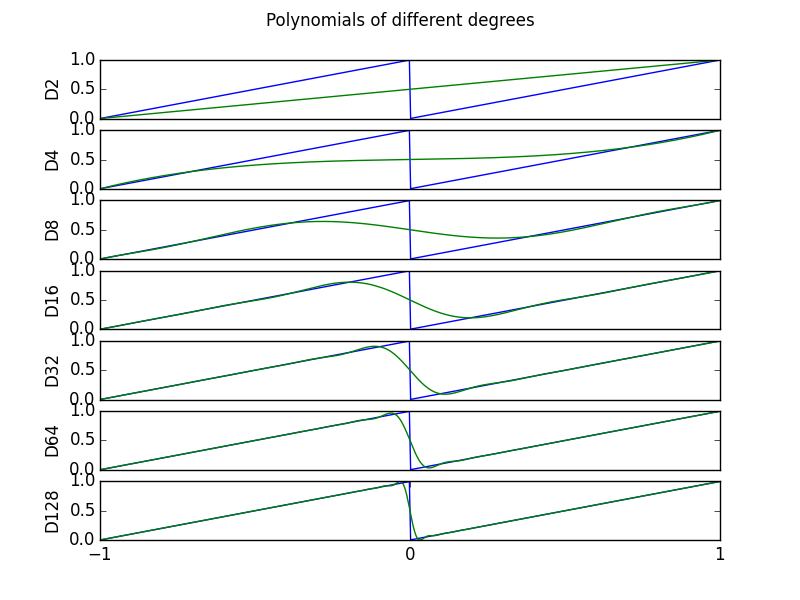
\includegraphics[scale = .75]{prob23.png}







\end{document}
